% =========== Dokumentgrundeinstellungen =================
\documentclass[a4paper,12pt]{scrreprt}
\usepackage[left= 3.0cm,right= 2.5cm,bottom= 4cm]{geometry}

% PDF informationen
\usepackage[pdftitle={Optimierung der Präklinischen Patientenbehandlung
durch Entwicklung einer Software zur Anleitung und
Beratung für Notfallsanitäter durch einen entfernten
Notarzt}, pdfsubject={}, pdfauthor={Maurice Müller}]{hyperref}

% Standart Packages
\usepackage[utf8]{inputenc}
\usepackage[ngerman]{babel}
\usepackage[T1]{fontenc}
\usepackage{graphicx}
\usepackage{float}
\usepackage{graphicx, subfigure}
\graphicspath{{pics/}}
\usepackage{fancyhdr}
\usepackage{lmodern}
\usepackage{color}
\usepackage{transparent} 
\usepackage[printonlyused]{acronym}
\usepackage{url}
\usepackage{multibib}
\usepackage{tabularx}
\usepackage{booktabs} % Für schönere Tabellen

\renewcommand{\familydefault}{\sfdefault}
\usepackage{helvet}

\usepackage{setspace}
% nicht einrücken nach Absatz
\setlength{\parindent}{0pt}
\setstretch{1.25}
% =========== Kopf- und Fußzeile =================
\pagestyle{fancy}

\lhead{\slshape \nouppercase {\leftmark} }
\chead{}
\rhead{}

\lfoot{}
\cfoot{\thepage}
\rfoot{}
\renewcommand{\headrulewidth}{0.6pt}



% ============== Farben ================
\definecolor{BeuthMainColor}{rgb}{0,0.593,0.629}

\hypersetup{colorlinks = true}
\hypersetup{linkcolor = black}
\hypersetup{citecolor = black}
\hypersetup{filecolor = black}
\hypersetup{pagecolor = black}
\hypersetup{urlcolor = black}
% =========== Dokumentbeginn =================
\begin{document}
% Titelblatt   
\pagestyle{empty}

\begin{titlepage}
    \sffamily
    \centering
    \vspace*{-3.5cm} % Adjust the value as needed
    
\includegraphics[width=12cm]{BHT_Logo_og.png}
   

    {- Fachbereich VI Medien und Informatik -\par \vspace{0.5cm}
    im Studiengang\par Medieninformatik\par}
    \vspace{1.25cm}
 

    {\Large \bfseries{Optimierung der Präklinischen Patientenbehandlung durch Entwicklung einer
    Software zur Anleitung und Beratung für Notfallsanitäter durch einen entfernten
    Notarzt}\par}
	\vspace{1.25cm}
	
    
    \normalsize vorgelegt von \par\vspace{1.25cm}

	{\large \bfseries Maurice Müller} \par\vspace{0.1cm}
	 Matrikelnummer: S903866 \par \vspace{1.25cm}

    {\large zur Erlangung des akademischen Grades\par
    Master of Science (M.Sc.)\par}


    \vspace{1.0cm}
    {\normalsize  Eingereicht:  22. Januar 2023\par}
   

   
    % Bottom of the page
    \vfill
    \begin{center}
      { \normalsize
        Betreuer:  \hspace{12mm} Prof. Dr. Stefan Edlich\\
        Gutachter:\hspace{12mm} Prof. Dr. Stefan Edlich\\
       }
    \end{center} 



\end{titlepage}

% part im Inhaltsverzeichnis nicht nummerieren


\pagestyle{fancy}
% Seitennummerierung neu beginnen, Zahlen[arabic],röm.Zahlen
\pagenumbering{roman}


\clearpage

%Erklärung
\newpage
\include{Erklärung}


%Danksagungen
\newpage
\section*{Danksagung}
Lorem ipsum dolor sit amet, consetetur sadipscing elitr,
sed diam nonumy eirmod tempor invidunt ut labore et dolore magna aliquyam erat, 
sed diam voluptua. At vero eos et accusam et justo duo dolores et ea rebum. \\

Stet clita kasd gubergren, no sea takimata sanctus est Lorem ipsum dolor sit amet. 
Lorem ipsum dolor sit amet, consetetur sadipscing elitr, sed diam nonumy eirmod tempor invidunt ut labore et dolore magna 
aliquyam erat, sed diam voluptua. At vero eos et accusam et justo duo dolores et ea rebum. Stet clita kasd gubergren, no sea 
takimata sanctus est Lorem ipsum dolor sit amet. \\

Vielen Dank 



%Zusammenfassung
\newpage
\section*{Abstract}

The present master's thesis is dedicated to the
 development of an innovative software designed to 
facilitate the remote treatment of patients. The primary
objective is not only to enhance the effectiveness of patient
care but also to significantly alleviate the workload of the healthcare
personnel through the utilization of this software. By implementing this 
advanced solution, the thesis aims to contribute to the efficiency improvement 
in the healthcare sector and ensure an enhanced level of patient care.





%Inhaltsverzeichnis
\newpage
\pagestyle{fancy}
\tableofcontents


% =========== Abkürzungsverzeichnis =================
\newpage
\pagestyle{empty}

\addcontentsline{toc}{chapter}{Abkürzungsverzeichnis}
\include{Abkürzungsverzeichnis}


\addchap{Glossar}

\textbf{WebRTC-Verbindung} \\
WebRTC steht für "Web Real-Time Communication" 
und ist eine offene Webtechnologie, die Echtzeitkommunikation 
über Webbrowser ermöglicht \\

\textbf{iOS} \\
iOS ist das mobile Betriebssystem von Apple, 
entwickelt für Geräte wie iPhones und iPads. \\

\textbf{Mobile Einsatzdokumentation} \\
MDE steht für Mobile Einsatzdokumentation und ermöglicht die digitale Erfassung von Daten während eines Einsatzes.

\pagestyle{fancy}

%Hauptteil

\newpage
\pagenumbering{arabic}
\chapter{Einleitung}


\section{Motivation}
Die vorliegende Masterarbeit strebt die Optimierung des Informationsaustauschs zwischen Notfallsanitätern und Notärzten an, um eine erstklassige Patientenversorgung zu gewährleisten und den beratenden Arzt bestmöglich zu unterstützen. Das zentrale Ziel besteht darin, eine Software zu entwickeln, die es ermöglicht, den Arzt virtuell am Einsatzgeschehen teilhaben zu lassen. In einem digitalen Paradigmenwechsel soll das bisherige Konzept, bestehend aus einem \ac{NEF} und einem \ac{RTW}, transformiert werden. Diese Digitalisierung ermöglicht die Alarmierung eines virtuellen NEF für den Einsatz. Der Notarzt auf dem virtuellen NEF erhält remote Zugriff auf sämtliche Einsatzdaten, indem eine browserbasierte Anwendung entwickelt wird. Diese Anwendung gewährt dem Notarzt Zugriff auf die digitale Einsatzdokumentation, den Defibrillator, Beatmungsgeräte und Leitstellendaten. Darüber hinaus wird eine WebRTC-Verbindung zu den fest installierten Kameras im Rettungswagen und den mobilen Geräten der Notfallsanitäter hergestellt. Diese bahnbrechende Initiative verspricht eine effizientere Koordination und Kommunikation im Rettungswesen, um letztendlich die Qualität der medizinischen Notfallversorgung zu verbessern.


\section{Aufbau der Arbeit}

In den kommenden Kapiteln werden die grundlegenden Aspekte dieser Arbeit ausführlich erläutert. Dabei werden sowohl fachliche Grundlagen, auf die die Arbeit aufbaut, als auch technische Grundlagen, auf die die Arbeit aufsetzt, behandelt. \\

In den fachlichen Grundlagen wird detailliert auf den Ablauf des Einsatzgeschehens eingegangen. Ziel ist es, dem Leser einen umfassenden Überblick über die Funktionsweise der präklinischen Patientenbehandlung zu vermitteln. Hierbei wird im Besonderen aufgezeigt, wie die einzelnen Schritte des Einsatzablaufs ineinandergreifen, um eine bestmögliche Versorgung der Patienten sicherzustellen. \\

Zudem wird auf die technische Ausstattung am Einsatzort, am Fahrzeug sowie die Ausrüstung des Rettungssanitäters/Notfallsanitäters eingehend erläutert. Dies dient dazu, dem Leser einen umfassenden Einblick zu verschaffen, um nachvollziehen zu können, auf welchen Geräten welche Informationen verfügbar sind.  \\


In den technischen Grundlagen werden hingegen die verwendeten Technologien betrachtet. Dabei wird die Software in ihre einzelnen Komponenten aufgebrochen und jede Komponente anschließend detailliert beleuchtet. \\

Es erfolgt eine ausführliche Erläuterung der mobilen Endgeräte am Einsatzort sowie der darauf verwendeten Softwaretechnologien, die die Anwendung ermöglichen. Ebenso werden die erforderlichen Schnittstellentechnologien zu Drittsystemen beschrieben, um Zugriff auf einsatztaktische Daten zu erhalten.\\

Die \ac{TNA-Z} und ihr Aufbau, einschließlich der eingesetzten Softwaretechnologien, werden eingehend erläutert. Abschließend wird in den Grundlagen ausführlich über die eingesetzte Software im Backend berichtet, einschließlich der Struktur und des Aufbaus der Infrastruktur. Dabei wird unter anderem aufgezeigt, wie mit Hilfe von Microservices und Kubernetes eine hohe Verfügbarkeit erreicht wird.\\

In den nachfolgenden Kapiteln werden Lorem ipsum dolor sit amet, consetetur sadipscing elitr, sed diam nonumy eirmod tempor invidunt ut labore et dolore magna aliquyam erat, sed diam voluptua. At vero eos et accusam et justo duo dolores et ea rebum. Stet clita kasd gubergren, no sea takimata sanctus est Lorem ipsum dolor sit amet. Lorem ipsum dolor sit amet, consetetur sadipscing elitr, sed diam nonumy eirmod tempor invidunt ut labore et dolore magna aliquyam erat, sed diam voluptua. At vero eos et accusam et justo duo dolores et ea rebum. Stet clita kasd gubergren, no sea takimata sanctus est Lorem ipsum dolor sit amet. \\


\section{Ziel der Arbeit}
Das Ziel dieser Studie besteht darin,
den Informationsaustausch zwischen Notfallsanitätern und Notärzten zu optimieren, um eine bestmögliche Patientenversorgung sicherzustellen und den konsultierenden Arzt bestmöglich zu unterstützen. Dies soll durch die Entwicklung einer Software erreicht werden, die es ermöglicht, den Arzt virtuell am Einsatzgeschehen teilhaben zu lassen. In kurzen Worten gesagt, das bestehende Konzept mit einem \ac{NEF} und einem \ac{RTW} soll digitalisiert werden.

Durch diese Digitalisierung wird es möglich, einen virtuellen \ac{NEF} für den Einsatz zu aktivieren. Der Notarzt auf dem virtuellen \ac{NEF} erhält remote Zugriff auf sämtliche Einsatzdaten. Hierfür wird eine browserbasierte Anwendung entwickelt, die dem Notarzt den Zugriff auf die digitale Einsatzdokumentation, den Defibrillator, Beatmungsgeräte und Leitstellendaten ermöglicht. Zusätzlich wird eine WebRTC-Verbindung zu den fest installierten Kameras im Rettungswagen und den mobilen Geräten der Notfallsanitäter hergestellt.
\\

Daraus ergeben sich die folgenden Hypothesen:

\begin{itemize}
    \item \textbf{1 Hypothese}: Der Einsatz einer TNA-Software reduziert den Personalmangel in der präklinischen Notfallversorgung.
    
    \item \textbf{2 Hypothese}: Die präklinische Patientenversorgung wird durch den Einsatz der Software signifikant verbessert.
    
    \item \textbf{3 Hypothese}: Es werden zusätzliche Ressourcen in Kliniken geschaffen.
  \end{itemize}

\newpage
\chapter{Grundlagen} 
Im Kapitel Grundlagen erfolgt eine fachliche Beschreibung 
des Einsatzumfelds der Software. Dabei wird der Ablauf eines 
Rettungseinsatzes sowie die vorhandenen medizinischen Geräte erläutert. 
Im Anschluss werden die Komponenten der Software näher betrachtet, insbesondere
unter Berücksichtigung der verwendeten Technologien und Frameworks.

\section{Aufbau Rettungsdiensteinsatz}
Ein Rettungsdiensteinsatz in Deutschland beginnt mit einem Notruf bei der
Notrufnummer 112 oder der örtlichen Rettungsleitstelle. Die Leitstelle
entscheidet über die Art des Einsatzes und alarmiert die entsprechenden
Rettungsmittel. Zwei wichtige Komponenten des Rettungsdienstes sind dabei
das \ac{NEF} und der \ac{RTW}.
Das \ac{NEF}, besetzt mit einem Notarzt und oft auch einem Rettungsassistenten
oder Notfallsanitäter, hat die Aufgabe, den Notarzt so schnell wie möglich
zum Einsatzort zu bringen, um eine qualifizierte medizinische Versorgung
sicherzustellen. Parallel dazu wird der \ac{RTW}, in der Regel besetzt mit
Rettungsassistenten oder Notfallsanitätern, zum Einsatzort geschickt.
Der RTW übernimmt primär den Transport von Patienten. \\

Am Einsatzort erfolgt eine enge Zusammenarbeit zwischen dem Notarzt
und dem Notfallsanitäter im \ac{RTW}.Der Notfallsanitäter übernimmt die 
Erstversorgung des Patienten und bereitet alles für den Transport vor.
Der Notarzt unterstützt den Notfallsanitäter und übernimmt die
medizinische Verantwortung. Die Zusammenarbeit basiert auf klaren
Handlungsanweisungen und Protokollen. \\

Nach der Erstversorgung entscheiden Notarzt und Notfallsanitäter
gemeinsam über den weiteren Transport des Patienten, entweder zur nächsten
geeigneten Klinik oder zu einer spezialisierten Einrichtung, wenn erforderlich.
Die Abstimmung zwischen \ac{NEF} und \ac{RTW} sowie die Koordination zwischen Notarzt
und Notfallsanitäter sind entscheidend, um eine optimale Patientenversorgung
zu gewährleisten.\\

Der Ablauf eines Rettungsdiensteinsatzes beruht auf einer klaren Struktur
und effektiven Kommunikation, um in Notfallsituationen rasch und professionell
handeln zu können.\\

\section{Medizingeräte und Vitaldaten}
Die eingesetzte Medizintechnik am Einsatzort spielt 
eine entscheidende Rolle bei der Gewährleistung einer effizienten
und qualitativ hochwertigen präklinischen Versorgung von Patienten. 
Verschiedene medizinische Geräte und Instrumente werden gezielt eingesetzt, 
um eine schnelle Diagnosestellung, Stabilisierung des Patienten und die 
notwendigen lebenserhaltenden Maßnahmen zu ermöglichen.\\

Ein unverzichtbares Instrument ist der Defibrillator, der zur Behandlung
lebensbedrohlicher Herzrhythmusstörungen eingesetzt wird.\\

Zur medizinischen Ausstattung am Einsatzort gehören auch tragbare
Monitore zur kontinuierlichen Überwachung von Vitalparametern wie
Herzfrequenz, Blutdruck und Sauerstoffsättigung. Diese Informationen
sind entscheidend für die Einschätzung des Patientenzustands und die
Anpassung der therapeutischen Maßnahmen.\\

Aktuell verfügen die meisten dieser eingesetzten Geräte bereits
über hochperformante Datenschnittstellen, um die erfassten Informationen
an Dritte weiterzugeben. Dabei basieren die meisten Schnittstellen in der
Regel auf der Bluetooth-Technologie. Neuere Geräte setzen vermehrt auf
Cloud-Schnittstellen. In Kombination mit prioritisierten SIM-Karten werden
die Daten der Geräte so dezentral verteilt.\\

\section{Frontend Komponenten}
Die im Frontend eingesetzten Komponenten müssen den
anspruchsvollen Bedingungen im Einsatz standhalten und eine
benutzerfreundliche Bedienung für Rettungskräfte gewährleisten. 
Zusätzlich ist eine schnelle Austauschbarkeit im Falle eines Defekts
erforderlich, weshalb hochverfügbare Hardware notwendig ist. 
Aus diesem Grund wurde die Entscheidung getroffen, auf Consumer-Geräte 
zurückzugreifen, die zweifelsohne die zuvor genannten Kriterien erfüllen. 
Da die Geräte am Einsatzort ein essenzieller Bestandteil sind, um mit der 
\ac{TNA-Z} zu kommunizieren, wurde besonderer Wert auf hohe Flexibilität gelegt. 
Die Wahl fiel hier auf Apple- und Android-Telefone, die mit der in dieser Arbeit 
entwickelten Software bespielt werden. Zur Kostenoptimierung und schnelleren
Reaktion auf Änderungen wurde das Framework React Native gewählt. Zudem 
gewinnt Die plattformübergreifende Entwicklung zunehmend an akzeptanz in der Anwendungsentwicklung \cite{bertels2023kategorisierung}.\\

Für die Software des Notarztes, der sich an einem entfernten Ort befindet, 
wurde entschieden, eine Browseranwendung bereitzustellen. Der Vorteil einer
Browseranwendung liegt in der Entkopplung von der Hardware und der damit
verbundenen Flexibilität. Entschieden wurde sich für das Framework Next.js, u.a.
spielte auch die fachliche Nähe zu React Native eine entscheidende Rolle.\\

\subsection{React-Native}
React Native hat sich zu einer der führenden Plattformen für die
Entwicklung plattformübergreifender mobiler Anwendungen entwickelt. 
Durch die Nutzung von JavaScript/TypeScript und React ermöglicht es 
Entwicklern, hochperformante native Apps für iOS und Android zu erstellen. \\

Einer der Hauptvorteile von React Native ist die Fähigkeit, dass 
React Native JavaScript/TypeScript-Code in echten nativen Code komeliert.
Dadurch sehen und fühlen sich die erstellten Apps so an, als wären sie 
mit nativen Entwicklungstechnologien erstellt worden.\\

Ein weiteres entscheidendes Merkmal ist die Möglichkeit der 
Wiederverwendung von Code zwischen verschiedenen Plattformen.
Der Großteil des Codes kann plattformübergreifend verwendet werden,
was die Entwicklungseffizienz erheblich steigert und konsistente 
Funktionalitäten auf verschiedenen Geräten gewährleistet.\\

Die Architektur von React Native fördert die Modulstruktur, 
was bedeutet, dass verschiedene Funktionen in separate Module aufgeteilt 
werden können. Die React Native-Community hat eine breite Palette 
von vorgefertigten Modulen geschaffen, die den Entwicklungsprozess 
beschleunigen und den Funktionsumfang erweitern.\\

Der grundlegende Aufbau von React Native basiert auf React-Komponenten,
die Teile der Benutzeroberfläche repräsentieren und sowohl einfach
als auch komplex sein können. 
JSX, eine Syntaxerweiterung für JavaScript, wird verwendet, um Benutzeroberflächenelemente 
zu deklarieren, wodurch die Erstellung von UI-Komponenten auf eine 
intuitive Weise erfolgt.\\

\begin{figure}[H]
    \centering
    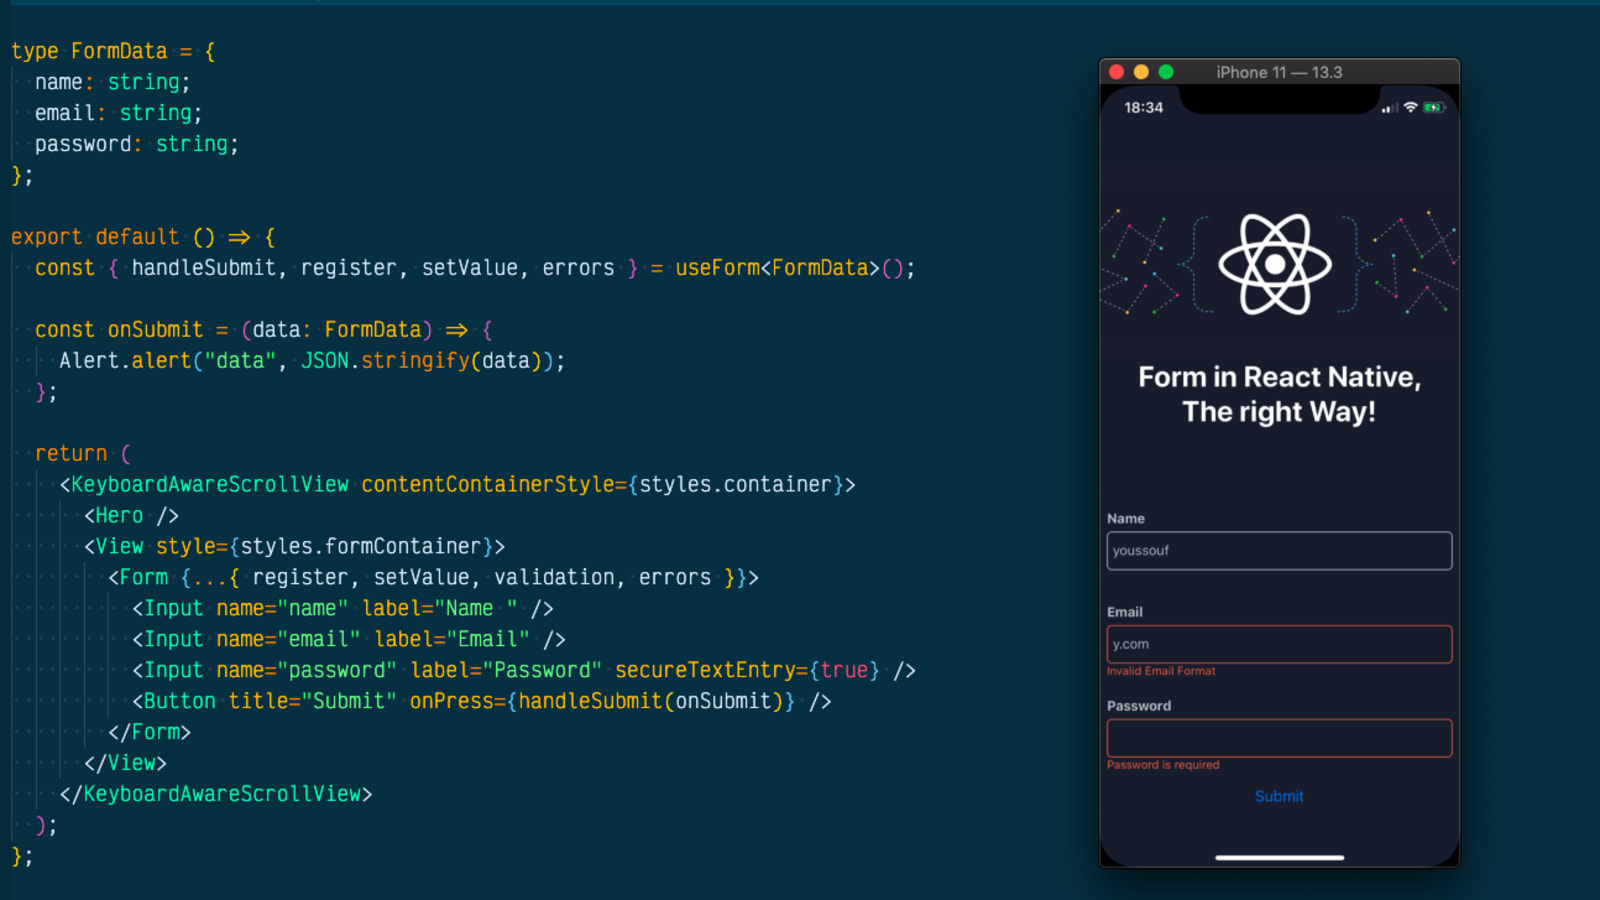
\includegraphics[width=1.0\textwidth]{ReactNative}
    \caption{Darstellung Code und UI mit React-Native[Quelle: \cite{ReactNativeCode}]}
    \label{img:ReactNative}
\end{figure}

Die Styling-Sprache in React Native ähnelt CSS, bietet jedoch nur eine 
begrenzte Menge an Styles. Dies stellt sicher, dass die Apps 
auf verschiedenen Plattformen konsistent aussehen, während 
gleichzeitig plattformspezifische Styles angewendet werden können.\\

\subsection{Next.js}
Lorem ipsum dolor sit amet, consetetur sadipscing
elitr, sed diam nonumy eirmod tempor invidunt ut labore
et dolore magna aliquyam erat, sed diam voluptua. At vero eos et
accusam et justo duo dolores et ea rebum. Stet clita kasd gubergren, 
no sea takimata sanctus est Lorem ipsum dolor sit amet. Lorem ipsum dolor 
sit amet, consetetur sadipscing elitr, sed diam nonumy eirmod tempor 
invidunt ut labore et dolore magna aliquyam erat, sed diam voluptua. 
At vero eos et accusam et justo duo dolores et ea rebum. Stet clita kasd 
gubergren, no sea takimata sanctus est Lorem ipsum dolor sit amet.

\section{Backend Komponenten}
Lorem ipsum dolor sit amet, consetetur sadipscing
elitr, sed diam nonumy eirmod tempor invidunt ut labore
et dolore magna aliquyam erat, sed diam voluptua. At vero eos et
accusam et justo duo dolores et ea rebum. Stet clita kasd gubergren, 
no sea takimata sanctus est Lorem ipsum dolor sit amet. Lorem ipsum dolor 
sit amet, consetetur sadipscing elitr, sed diam nonumy eirmod tempor 
invidunt ut labore et dolore magna aliquyam erat, sed diam voluptua. 
At vero eos et accusam et justo duo dolores et ea rebum. Stet clita kasd 
gubergren, no sea takimata sanctus est Lorem ipsum dolor sit amet.

\subsection{Microservices mit Java springboot}
Lorem ipsum dolor sit amet, consetetur sadipscing
elitr, sed diam nonumy eirmod tempor invidunt ut labore
et dolore magna aliquyam erat, sed diam voluptua. At vero eos et
accusam et justo duo dolores et ea rebum. Stet clita kasd gubergren, 
no sea takimata sanctus est Lorem ipsum dolor sit amet. Lorem ipsum dolor 
sit amet, consetetur sadipscing elitr, sed diam nonumy eirmod tempor 
invidunt ut labore et dolore magna aliquyam erat, sed diam voluptua. 
At vero eos et accusam et justo duo dolores et ea rebum. Stet clita kasd 
gubergren, no sea takimata sanctus est Lorem ipsum dolor sit amet.

\subsection{Authentifizierung}
Lorem ipsum dolor sit amet, consetetur sadipscing
elitr, sed diam nonumy eirmod tempor invidunt ut labore
et dolore magna aliquyam erat, sed diam voluptua. At vero eos et
accusam et justo duo dolores et ea rebum. Stet clita kasd gubergren, 
no sea takimata sanctus est Lorem ipsum dolor sit amet. Lorem ipsum dolor 
sit amet, consetetur sadipscing elitr, sed diam nonumy eirmod tempor 
invidunt ut labore et dolore magna aliquyam erat, sed diam voluptua. 
At vero eos et accusam et justo duo dolores et ea rebum. Stet clita kasd 
gubergren, no sea takimata sanctus est Lorem ipsum dolor sit amet.

\subsection{Kubernetes}
Lorem ipsum dolor sit amet, consetetur sadipscing
elitr, sed diam nonumy eirmod tempor invidunt ut labore
et dolore magna aliquyam erat, sed diam voluptua. At vero eos et
accusam et justo duo dolores et ea rebum. Stet clita kasd gubergren, 
no sea takimata sanctus est Lorem ipsum dolor sit amet. Lorem ipsum dolor 
sit amet, consetetur sadipscing elitr, sed diam nonumy eirmod tempor 
invidunt ut labore et dolore magna aliquyam erat, sed diam voluptua. 
At vero eos et accusam et justo duo dolores et ea rebum. Stet clita kasd 
gubergren, no sea takimata sanctus est Lorem ipsum dolor sit amet.


\newpage
\chapter{Anforderungen}

Dieses Kapitel beginnt mit einer Recherche über die aktuellen Prozesse 
eines Notfalleinsatzes und untersucht, an welcher Stelle der Einsatz von 
Telemedizin bereits angedacht oder in vereinfachter Form bereits in Betrieb ist. 
Die recherchierten Informationen wurden im Rahmen dieser 
Arbeit ermittelt und spiegeln den aktuellen Stand wider. 
Darüber hinaus werden die Erwartungen an die Anwendung 
aufgezeigt und in funktionale und nicht-funktionale 
Anforderungen aufgeteilt sowie thematisiert. Abschließend 
erfolgt eine Präzisierung der Anforderungen.

\section{Aktueller Stand Notfalleinsatz}

In Deutschland beginnt ein Notfalleinsatz, wie etwa bei einem gestürzten 
Patienten, mit einem Anruf bei der Notrufnummer 112. 
Der Anrufer beschreibt die Situation, und die 
Einsatzleitstelle bewertet diese Informationen, 
um angemessene Rettungskräfte zu entsenden. Sobald die 
Rettungskräfte am Einsatzort eintreffen, beurteilen sie 
den Gesundheitszustand des Patienten. Sie leisten Erste 
Hilfe und stabilisieren den Patienten. Dabei werden 
eventuelle Verletzungen versorgt, Vitalfunktionen 
kontrolliert und bei Bedarf lebensrettende Maßnahmen 
durchgeführt. Bei Bedarf wird der Patient anschließend in 
ein Krankenhaus transportiert, um eine weiterführende 
medizinische Versorgung zu gewährleisten. Jede Maßnahme 
wird sorgfältig entsprechend der medizinischen 
Dringlichkeit und der spezifischen Situation des Patienten 
ausgewählt und durchgeführt.\\

\begin{figure}[H]
    \centering
    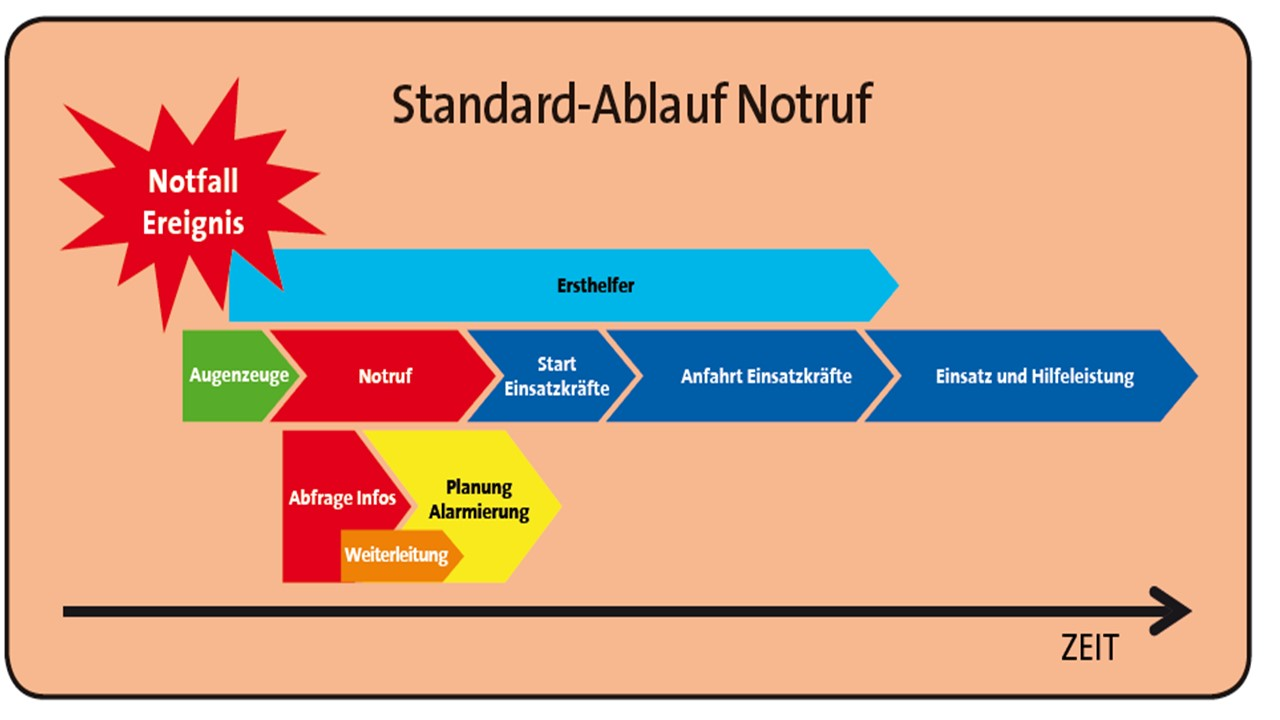
\includegraphics[width=1.0\textwidth]{Ablauf_Notruf}
    \caption{Abbildung eines Notfalleinsatzes.[Quelle: \cite{NotfallAblauf}]}
    \label{img:Ablauf_Notruf}
\end{figure}


Beim Zusammenspiel von Notfallsanitätern und Notärzten in 
Deutschland ergänzen sich beide Berufsgruppen. 
Notfallsanitäter treffen zuerst am Einsatzort ein, 
leisten Erste Hilfe und beginnen mit der Patientenversorgung. 
Sie haben eine umfassende Ausbildung und dürfen bestimmte 
medizinische Maßnahmen eigenständig durchführen. Wenn die 
Situation des Patienten es erfordert, wird zusätzlich ein Notarzt hinzugezogen. 
Dieser kann erweiterte medizinische Maßnahmen vornehmen, wie zum 
Beispiel das Verabreichen bestimmter Medikamente oder invasive Eingriffe. 
Gemeinsam stellen Notfallsanitäter und Notarzt die bestmögliche 
Versorgung des Patienten sicher.\\


Der Einsatz einer entfernten Unterstützung durch einen Notarzt, wie 
zum Beispiel telefonische Beratung, wird derzeit nicht 
praktiziert. Dies liegt unter anderem an Herausforderungen 
wie eingeschränkter Sprachqualität, Verständnisproblemen 
und rechtlichen Unsicherheiten bezüglich der Delegation 
medizinischer Maßnahmen. 

\section{Erwartungen an die TNA-Software}

Die Erwartungen an eine präklinische Telenotarzt-Software sind vielfältig.

Eine solche Software sollte eine intuitive Benutzeroberfläche besitzen, die selbst unter Stressbedingungen einfach zu bedienen ist. Ihre Funktionalität muss auf verschiedenen Geräten wie Tablets, Smartphones und Pc's gewährleistet sein, um eine breite Zugänglichkeit zu ermöglichen. Ein Kernaspekt der Software ist die Bereitstellung einer stabilen und sicheren Kommunikationsverbindung, die eine Video- und Audiokommunikation zwischen dem Telenotarzt und dem Rettungsdienstpersonal ermöglicht. Hierbei ist die Qualität der Übertragung entscheidend, um Fehldiagnosen und Missverständnisse zu vermeiden.

Wichtig ist auch die Fähigkeit der Software, patientenbezogene Daten effizient zu erfassen, zu speichern und zu verarbeiten. Dies umfasst Vitalparameter, Medikamentenlisten und Allergieinformationen.

Der Datenschutz und die Sicherheit der übertragenen medizinischen Daten haben oberste Priorität. Verschlüsselung der Datenübertragung und strenge Zugriffskontrollen sind unerlässlich, um die Privatsphäre der Patienten zu schützen. Zudem sollte die Software mit anderen medizinischen Systemen und Geräten interoperabel sein und eine flexible Architektur aufweisen, die Anpassungen an lokale Gegebenheiten und zukünftige technologische Entwicklungen ermöglicht.


\section{Anforderungsanalyse}


Dieses Kapitel widmet sich der ausführlichen Darstellung der verschiedenen Anforderungsarten der Applikation. 
Zunächst wird der Anwendungsfall durch ein aussagekräftiges Diagramm visualisiert. Im Anschluss daran folgt eine Erläuterung der User-Stories, 
die als Grundlage für die Ableitung der funktionalen Anforderungen dienen. Nachfolgend werden die nicht-funktionalen Anforderungen aufgeführt und detailliert 
beschrieben. Sowohl die funktionalen als auch die nicht-funktionalen Anforderungen werden in übersichtlichen Tabellen präsentiert, die eine klare Priorisierung 
und Zusammenfassung der einzelnen Punkte ermöglichen. Das Kapitel schließt mit einer präzisen Abgrenzung der Anforderungen ab, die als Orientierung für die 
nachfolgenden Kapitel dient.


\subsection{Use-Cases der TNA-Software}

Im Folgenden werden zwei Use-Cases für die TNA-Software präsentiert, um deren Funktionalitäten und Anwendungsgebiete genauer zu erläutern und zu vertiefen. \\\\

\textbf{Use-Case 1:} Alamierung für den Telenotarzt \\

Dieser Use-Case konzentriert sich auf die Anwendung der TNA-Software zur Optimierung des Einsatzablaufs für Notfallsanitäter im präklinischen Bereich.

\textbf{Akteure}\\

\begin{itemize}
    \item Notfallsanitäter
    \item Telenotarzt
\end{itemize}

\textbf{Hauptablauf}\\


\begin{enumerate}
\item Der Notfallsanitäter erhält einen Einsatzauftrag von der Rettungsleitstelle.
\item Während der Anfahrt zum Einsatzort verwendet der Sanitäter eine Dokumentationssoftware, um Echtzeitinformationen über den Einsatzort, die Patientenhistorie und eventuelle spezielle Anforderungen zu erhalten.
\item Die Software bietet die Möglichkeit, bei bedarf unterstützung eines TNA anzufordern.
\item Bei angeforderter unterstützung, werden sämtliche Patientendaten, Vitalzeichen und Symptomen an die TNA Software übermittelt.
\item Aufgrundlage der informationen, werden in der TNA-Software handlungsanweisungen geladen.
\item Während des Einsatzes kann der TNA auf medizinische Referenzdaten und Protokolle über die Software zugreifen.
\item Nach der Patientenversorgung und dem Transport zum Krankenhaus erfolgt die digitale Dokumentation des Einsatzes über die TNA-Software.
\end{enumerate}


\textbf{Alternativablauf}\\
Bei Bedarf kann die Software in Echtzeit auf Änderungen in der Einsatzsituation reagieren und Vorschläge für alternative Behandlungsmaßnahmen oder den Transport zu einem speziellen Krankenhaus geben.\\

\textbf{Use-Case 2:} Virtuelle Arztkonsultation \\

Dieser Use-Case beschreibt, wie die TNA-Software eine virtuelle Arztkonsultation während eines Rettungseinsatzes ermöglicht.

\textbf{Akteure}\\

\begin{itemize}
    \item Notfallsanitäter
    \item Telenotarzt
\end{itemize}

\textbf{Hauptablauf}\\

\begin{enumerate}
\item Während eines komplexen Einsatzes mit unklarer Diagnose oder speziellen medizinischen Herausforderungen aktiviert der Notfallsanitäter die virtuelle Arztkonsultation über die TNA-Software.
\item Die Software stellt eine sichere WebRTC-Verbindung zwischen dem Notfallsanitäter vor Ort und einem bereitstehenden Fernarzt her.
\item Der Telenotarzt kann live über die in den Rettungsfahrzeugen installierten Kameras und die mobilen Geräte der Sanitäter auf die Einsatzsituation zugreifen.
\item Der Telenotarzt kann den Notfallsanitäter bei der Diagnosestellung, der Auswahl von Behandlungsmaßnahmen und der Entscheidung über den weiteren Verlauf des Einsatzes unterstützen.
\item Die TNA-Software ermöglicht die gemeinsame Nutzung von medizinischen Daten und Befunden in Echtzeit.
\item Nach Abschluss der virtuellen Konsultation und Behandlungsempfehlungen kann der Einsatz vor Ort fortgesetzt werden. 
\end{enumerate}

\textbf{Alternativablauf}\\
- Bei Bedarf kann die TNA-Software auch eine Übertragung von Vitaldaten und medizinischen Bildern an den Telenotarzt ermöglichen, um eine fundierte Diagnose zu erleichtern.\\

Diese erweiterte Darstellung der beiden Use-Cases verdeutlicht die vielfältigen Anwendungsgebiete und den Nutzen der TNA-Software im Bereich der präklinischen Notfallversorgung. Die Software bietet nicht nur Unterstützung für Notfallsanitäter vor Ort, sondern ermöglicht auch eine effektive Zusammenarbeit mit Telenotarzt, um die bestmögliche Patientenversorgung sicherzustellen.


\subsection{Funktionale Anforderungen}
Funktionale Anforderungen in der Softwareentwicklung beschreiben Funktionen, Verhaltensweisen oder Leistungen, die eine Software oder ein System erbringen muss. 
Sie definieren, was das System tun soll, in verschiedenen Szenarien und unter verschiedenen Bedingungen. \cite{braun2016nicht}\\

\begin{itemize}
    \item \textbf{FA\#01} Die Anwendung muss die Möglichkeit bieten, sich sowohl als Notfallsanitäter als auch als Notarzt anzumelden.
    \item \textbf{FA\#02} Lorem ipsum dolor sit amet, consetetur sadipscing elitr, sed diam nonumy eirmod tempor invidunt ut labore et dolore magna aliquyam erat, sed diam voluptua. At vero eos et accusam et
    \item \textbf{FA\#03} Lorem ipsum dolor sit amet, consetetur sadipscing elitr, sed diam nonumy eirmod tempor invidunt ut labore et dolore magna aliquyam erat, sed diam voluptua. At vero eos et accusam et
    \item \textbf{FA\#04} Lorem ipsum dolor sit amet, consetetur sadipscing elitr, sed diam nonumy eirmod tempor invidunt ut labore et dolore magna aliquyam erat, sed diam voluptua. At vero eos et accusam et
    \item \textbf{FA\#05} Lorem ipsum dolor sit amet, consetetur sadipscing elitr, sed diam nonumy eirmod tempor invidunt ut labore et dolore magna aliquyam erat, sed diam voluptua. At vero eos et accusam et

\end{itemize}

\subsection{Nicht funktionaleAnforderungen}
Nicht-funktionale Anforderungen beziehen sich auf die allgemeine Qualität und Eigenschaften eines Systems, die nicht direkt dessen spezifische Funktionen betreffen. Sie beschreiben, wie gut ein System funktionieren soll und legen Standards fest. \cite{bergsmann2004nicht}

\begin{itemize}
    \item \textbf{NFA\#01} Die Anwendung muss die fähigkeit besitzen, mit steigender Nutzerzahl oder Datenvolumen effizient umzugehen.
    \item \textbf{NFA\#02} Lorem ipsum dolor sit amet, consetetur sadipscing elitr, sed diam nonumy eirmod tempor invidunt ut labore et dolore magna aliquyam erat, sed diam voluptua. At vero eos et accusam et
    \item \textbf{NFA\#03} Lorem ipsum dolor sit amet, consetetur sadipscing elitr, sed diam nonumy eirmod tempor invidunt ut labore et dolore magna aliquyam erat, sed diam voluptua. At vero eos et accusam et
    \item \textbf{NFA\#04} Lorem ipsum dolor sit amet, consetetur sadipscing elitr, sed diam nonumy eirmod tempor invidunt ut labore et dolore magna aliquyam erat, sed diam voluptua. At vero eos et accusam et
    \item \textbf{NFA\#05} Lorem ipsum dolor sit amet, consetetur sadipscing elitr, sed diam nonumy eirmod tempor invidunt ut labore et dolore magna aliquyam erat, sed diam voluptua. At vero eos et accusam et

\end{itemize}

\subsection{Zusammenfassung und Priorisierung}

In diesem Kapitel erfolgt eine strukturierte und übersichtliche Darstellung der verschiedenen Anforderungen an das Projekt, sowohl der funktionalen als auch der nicht-funktionalen Art. Diese Anforderungen werden in tabellarischer Form präsentiert, um eine klare und zugängliche Übersicht zu gewährleisten.



\begin{table}[ht]
    \centering
    \begin{tabularx}{\textwidth}{@{}lX@{}}
    \toprule
    ID & Funktionale Anforderung \\ 
    \midrule
    FA\#01 & Benutzeranmeldung \\
    FA\#02 & Lorem ipsum dolor sit amet \\
    FA\#03 & Lorem ipsum dolor sit amet \\
    FA\#04 & Lorem ipsum dolor sit amet \\
    FA\#05 & Lorem ipsum dolor sit amet \\
    \bottomrule
    \end{tabularx}
    \caption{Tabellarische Übersicht der funktionalen Anforderungen}
    \label{tab:FA-tabelle}
    \end{table}

\begin{table}[ht]
    \centering
    \begin{tabularx}{\textwidth}{@{}lX@{}}
    \toprule
    ID & Nicht-funktionale Anforderung \\ 
    \midrule
    NFA\#01 & Skalierbarkeit \\
    NFA\#02 & Lorem ipsum dolor sit amet \\
    NFA\#03 & Lorem ipsum dolor sit amet \\
    NFA\#04 & Lorem ipsum dolor sit amet \\
    NFA\#05 & Lorem ipsum dolor sit amet \\
    \bottomrule
    \end{tabularx}
    \caption{Tabellarische Übersicht der Nicht-funktionalen Anforderungen}
    \label{tab: NFA-tabelle}
    \end{table}

\subsection{EingrenzungenNFAAnforderungen}
Lorem ipsum dolor sit amet, consetetur sadipscing elitr, sed diam nonumy eirmod tempor invidunt ut labore et dolore magna aliquyam erat, sed diam voluptua. At vero eos et accusam et justo duo dolores et ea rebum. Stet clita kasd gubergren, no sea takimata sanctus est Lorem ipsum dolor sit amet. Lorem ipsum dolor sit amet, consetetur sadipscing elitr, sed diam nonumy eirmod tempor invidunt ut labore et dolore magna aliquyam erat, sed diam voluptua. At vero eos et accusam et justo duo dolores et ea rebum. Stet clita kasd gubergren, no sea takimata sanctus est Lorem ipsum dolor sit amet. Lorem ipsum dolor sit amet, consetetur sadipscing elitr, sed diam nonumy eirmod tempor invidunt ut labore et dolore magna aliquyam erat, sed diam voluptua. At vero eos et accusam et justo duo dolores et ea rebum. Stet clita kasd gubergren, no sea takimata sanctus est Lorem ipsum dolor sit amet.   
Duis autem vel eum iriure dolor in hendrerit in vulputate velit esse molestie consequat, vel illum dolore eu feugiat nulla facilisis at vero eros et accumsan et iusto odio dignissim qui blandit praesent luptatum zzril delenit augue duis dolore te feugait nulla facilisi. Lorem ipsum dolor sit amet,





\newpage

\chapter{Konzeption und Entwurf}
Lorem ipsum dolor sit amet, consetetur sadipscing
elitr, sed diam nonumy eirmod tempor invidunt ut labore
et dolore magna aliquyam erat, sed diam voluptua. At vero eos et
accusam et justo duo dolores et ea rebum. Stet clita kasd gubergren, 
no sea takimata sanctus est Lorem ipsum dolor sit amet. Lorem ipsum dolor 
sit amet, consetetur sadipscing elitr, sed diam nonumy eirmod tempor 
invidunt ut labore et dolore magna aliquyam erat, sed diam voluptua. 
At vero eos et accusam et justo duo dolores et ea rebum. Stet clita kasd 
gubergren, no sea takimata sanctus est Lorem ipsum dolor sit amet.

\section{Aufbau und Architektur der TNA-Software}


Die TNA-Software besteht aus mehreren Softwarekomponenten, um eine reibungslose Zusammenarbeit zwischen Notfallsanitätern und Notärzten sicherzustellen. Es ist von entscheidender Bedeutung, möglichst viele Daten am Einsatzort zu erfassen und diese bestmöglich für den entfernten Zugriff durch den Notarzt aufzubereiten. Da sich die Einsatzkräfte in stressigen Situationen befinden, ist es unerlässlich, die Benutzeroberfläche (UI) der Softwarekomponenten am Einsatzort zu optimieren. Die Stabilität der Datenübertragung spielt ebenfalls eine wichtige Rolle.

Um all diese Anforderungen zu erfüllen, werden folgende Softwarekomponenten in der TNA-Software eingesetzt:\\

\textbf{Schnistelle \ac{MDE}:}\\
Die Schnittstelle zum MDE ermöglicht den Zugriff auf zusätzliche Daten und reduziert den Schulungsaufwand.
Lorem ipsum dolor sit amet, consetetur sadipscing elitr, sed diam nonumy eirmod tempor invidunt ut labore et dolore magna aliquyam erat, sed diam voluptua. At vero eos et accusam et justo duo dolores et ea rebum. Stet clita kasd gubergren, no sea takimata sanctus est Lorem ipsum dolor sit amet. Lorem ipsum dolor sit amet, consetetur sadipscing elitr, sed diam nonumy eirmod tempor invidunt ut labore et dolore magna aliquyam erat, sed diam voluptua. At vero eos et accusam et justo duo dolores et ea rebum. Stet clita kasd gubergren, no sea takimata sanctus est Lorem ipsum dolor sit amet.\\

\textbf{Smartphone Anwendung}\\
Das Smartphone soll eine schnellere Kommunikation ermöglichen und beispielsweise dazu genutzt werden, mit dem TNA zu kommunizieren oder rudimentäre Daten auszutauschen.\\


\textbf{Web Anwendung}\\

Die Webanwendung stellt sozusagen das Fenster zur Einsatzstelle für den TNA dar. Dadurch hat er die Möglichkeit, auf die Daten des Patienten zuzugreifen, mit dem Patienten zu sprechen oder Anweisungen an das Rettungsdienstpersonal zu delegieren.\\

\textbf{Backend}\\


Das Backend wird sich aus mehreren Services zusammensetzen und in einer Kubernetes-Cloud bereitgestellt werden. Es muss hochverfügbare Services bereitstellen, die Daten zwischen den einzelnen Clients austauschen und archivieren.\\


\section{Eingesetzte Technologien}
Lorem ipsum dolor sit amet, consetetur sadipscing elitr, sed diam nonumy eirmod tempor invidunt ut labore et dolore magna aliquyam erat, sed diam voluptua. At vero eos et accusam et justo duo dolores et ea rebum. Stet clita kasd gubergren, no sea takimata sanctus est Lorem ipsum dolor sit amet. Lorem ipsum dolor sit amet, consetetur sadipscing elitr, sed diam nonumy eirmod tempor invidunt ut labore et dolore magna aliquyam erat, sed diam voluptua. At vero eos et accusam et justo duo dolores et ea rebum. Stet clita kasd gubergren, no sea takimata sanctus est Lorem ipsum dolor sit amet. Lorem ipsum dolor sit amet, consetetur sadipscing elitr, sed diam nonumy eirmod tempor invidunt ut labore et dolore magna aliquyam erat, sed diam voluptua. At vero eos et accusam et justo duo dolores et ea rebum. Stet clita kasd gubergren, no sea takimata sanctus est Lorem ipsum dolor sit amet.

\section{Datenbankarchitektur}
Lorem ipsum dolor sit amet, consetetur sadipscing elitr, sed diam nonumy eirmod tempor invidunt ut labore et dolore magna aliquyam erat, sed diam voluptua. At vero eos et accusam et justo duo dolores et ea rebum. Stet clita kasd gubergren, no sea takimata sanctus est Lorem ipsum dolor sit amet. Lorem ipsum dolor sit amet, consetetur sadipscing elitr, sed diam nonumy eirmod tempor invidunt ut labore et dolore magna aliquyam erat, sed diam voluptua. At vero eos et accusam et justo duo dolores et ea rebum. Stet clita kasd gubergren, no sea takimata sanctus est Lorem ipsum dolor sit amet. Lorem ipsum dolor sit amet, consetetur sadipscing elitr, sed diam nonumy eirmod tempor invidunt ut labore et dolore magna aliquyam erat, sed diam voluptua. At vero eos et accusam et justo duo dolores et ea rebum. Stet clita kasd gubergren, no sea takimata sanctus est Lorem ipsum dolor sit amet.

\section{Benutzeroberflächen und Design}
Lorem ipsum dolor sit amet, consetetur sadipscing elitr, sed diam nonumy eirmod tempor invidunt ut labore et dolore magna aliquyam erat, sed diam voluptua. 
At vero eos et accusam et justo duo dolores et ea rebum. Stet clita kasd gubergren, no sea takimata sanctus est Lorem ipsum dolor sit amet. Lorem ipsum dolor 
sit amet, consetetur sadipscing elitr, sed diam nonumy eirmod tempor invidunt ut labore et dolore magna aliquyam erat, sed diam voluptua. At vero eos et accusam 

\begin{figure}[H]
    \centering
    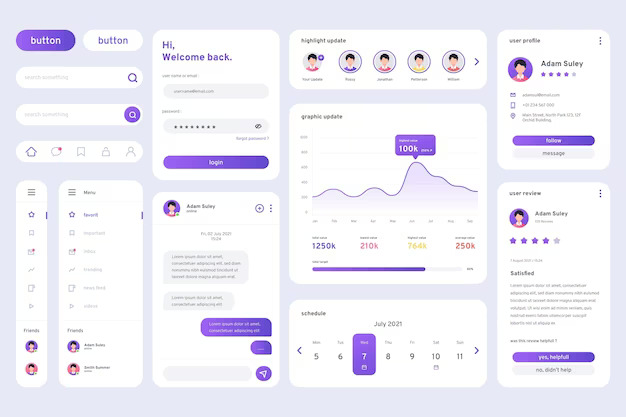
\includegraphics[width=1.0\textwidth]{TNAUI}
    \caption{Abbildung UI TNA Zentrale}
    \label{img:TNAUI}
\end{figure}

et justo duo dolores et ea rebum. Stet clita kasd gubergren, no sea takimata sanctus est Lorem ipsum dolor sit amet. Lorem ipsum dolor sit amet, consetetur sadipscing 
elitr, sed diam nonumy eirmod tempor invidunt ut labore et dolore magna aliquyam erat, sed diam voluptua. At vero eos et accusam et justo duo dolores et ea rebum. Stet 
clita kasd gubergren, no sea takimata sanctus est Lorem ipsum dolor sit amet.

\newpage

\chapter{Implementierung}
Lorem ipsum dolor sit amet, consetetur sadipscing
elitr, sed diam nonumy eirmod tempor invidunt ut labore
et dolore magna aliquyam erat, sed diam voluptua. At vero eos et
accusam et justo duo dolores et ea rebum. Stet clita kasd gubergren, 
no sea takimata sanctus est Lorem ipsum dolor sit amet. Lorem ipsum dolor 
sit amet, consetetur sadipscing elitr, sed diam nonumy eirmod tempor 
invidunt ut labore et dolore magna aliquyam erat, sed diam voluptua. 
At vero eos et accusam et justo duo dolores et ea rebum. Stet clita kasd 
gubergren, no sea takimata sanctus est Lorem ipsum dolor sit amet.


\section{Frontend-Komponentenentwicklung}


In diesem Kapitel wird ausführlich auf die Implementierung der Frontend-Komponenten eingegangen, wobei grundlegende Bestandteile detailliert erläutert werden

\subsection{Entwicklung Smartphone Anwendung}

Die Smartphone-Anwendung soll, wie zuvor beschrieben, eine möglichst große Zielgruppe erreichen. Um dieses Ziel zu erreichen, setzt die Anwendung auf React Native. Die Implementierung der Anwendung konzentrierte sich auf die folgenden Bestandteile.
Lorem ipsum dolor sit amet, consetetur sadipscing elitr, sed diam nonumy eirmod tempor invidunt ut labore et dolore magna aliquyam erat, sed diam voluptua. At vero eos et accusam et justo duo dolores et ea rebum. Stet clita kasd gubergren, no sea takimata sanctus est Lorem ipsum dolor sit amet. Lorem ipsum dolor sit amet, consetetur sadipscing elitr, sed diam nonumy eirmod tempor invidunt ut labore et dolore magna aliquyam erat, sed diam voluptua. At vero eos et accusam et justo duo dolores et ea rebum. Stet clita kasd gubergren, no sea takimata sanctus est Lorem ipsum dolor sit amet.

\begin{figure}[H]
    \centering
    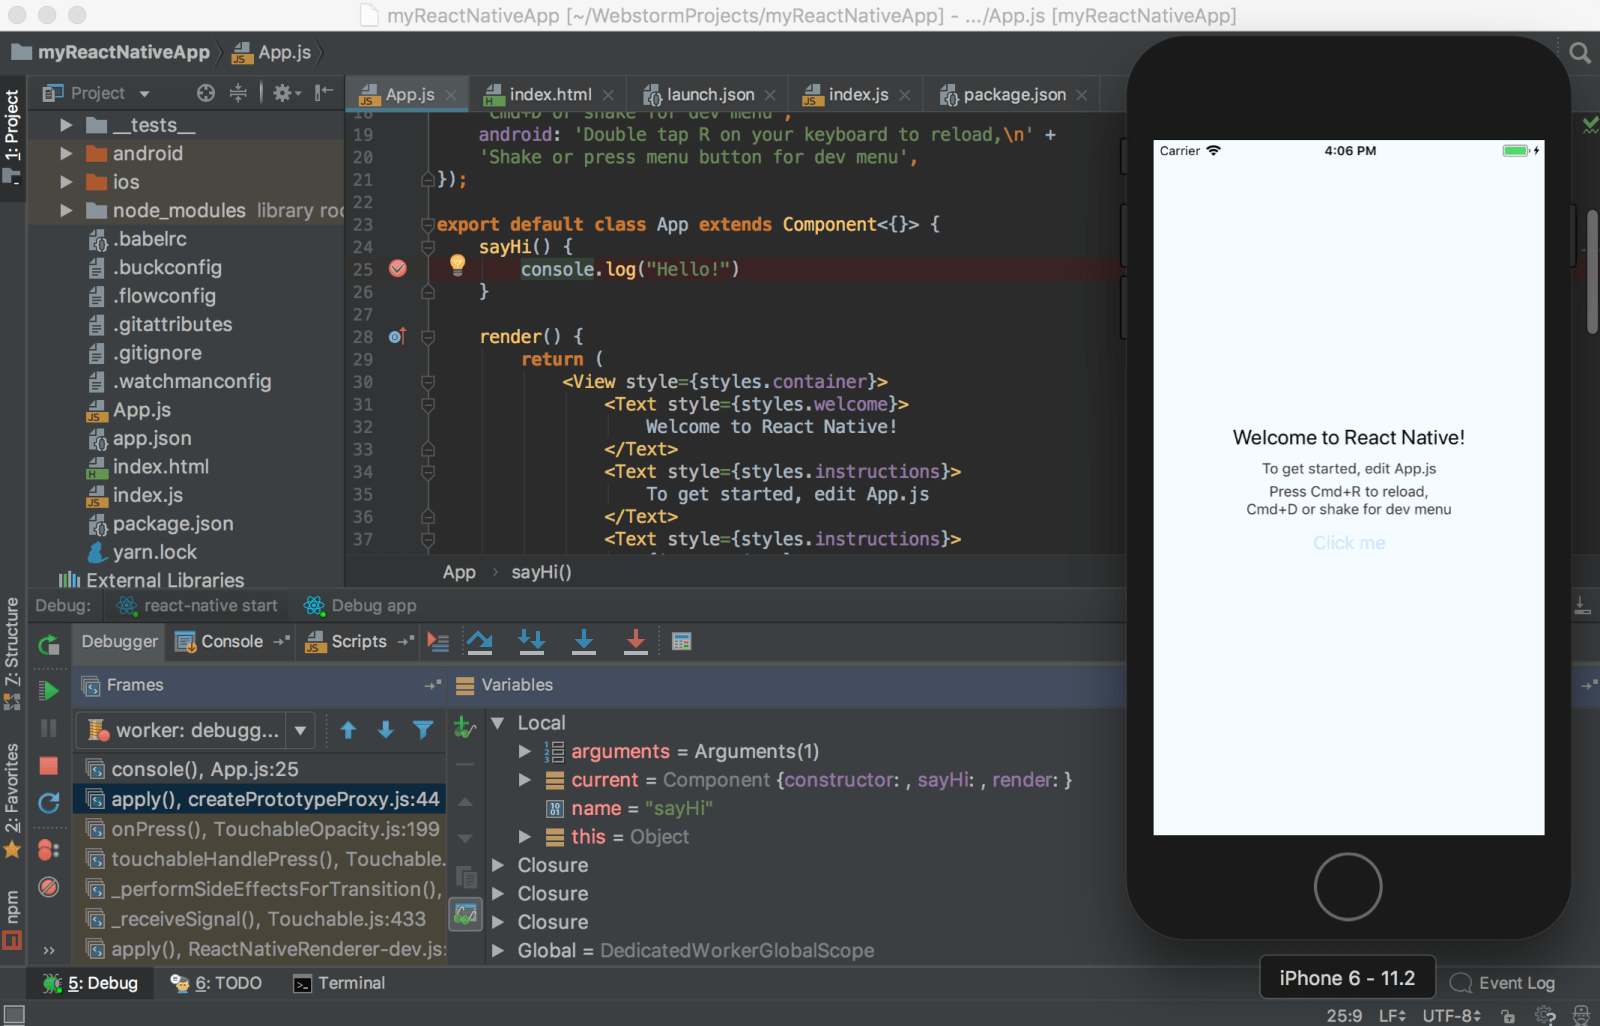
\includegraphics[width=1.0\textwidth]{ReactEnv}
    \caption{Entwicklungsumgebung für React Native}
    \label{img:ReactEnv}
\end{figure}

Lorem ipsum dolor sit amet, consetetur sadipscing elitr, sed diam nonumy eirmod tempor invidunt ut labore et dolore magna aliquyam erat, sed diam voluptua. At vero eos et accusam et justo duo dolores et ea rebum. Stet clita kasd gubergren, no sea takimata sanctus est Lorem ipsum dolor sit amet. Lorem ipsum dolor sit amet, consetetur sadipscing elitr, sed diam nonumy eirmod tempor invidunt ut labore et dolore magna aliquyam erat, sed diam voluptua. At vero eos et accusam et justo duo dolores et ea rebum. Stet clita kasd gubergren, no sea takimata sanctus est Lorem ipsum dolor sit amet.

\subsection{Entwicklung der Telenotarzt Zentrale}


Die Telenotarzt-Zentrale wird größtenteils stationär betrieben und erfordert eine möglichst hohe Informationsdichte. Die Anwendung wird mithilfe von React umgesetzt und setzt auf die folgenden Bestandteile:
Lorem ipsum dolor sit amet, consetetur sadipscing elitr, sed diam nonumy eirmod tempor invidunt ut labore et dolore magna aliquyam erat, sed diam voluptua. At vero eos et accusam et justo duo dolores et ea rebum. Stet clita kasd gubergren, no sea takimata sanctus est Lorem ipsum dolor sit amet. Lorem ipsum dolor sit amet, consetetur sadipscing elitr, sed diam nonumy eirmod tempor invidunt ut labore et dolore magna aliquyam erat, sed diam voluptua. At vero eos et accusam et justo duo dolores et ea rebum. Stet clita kasd gubergren, no sea takimata sanctus est Lorem ipsum dolor sit amet.

\begin{figure}[H]
    \centering
    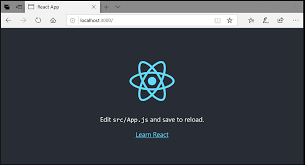
\includegraphics[width=1.0\textwidth]{rectWebEnv}
    \caption{Entwicklungsumgebung für React (Web)}
    \label{img:rectWebEnv}
\end{figure}

Lorem ipsum dolor sit amet, consetetur sadipscing elitr, sed diam nonumy eirmod tempor invidunt ut labore et dolore magna aliquyam erat, sed diam voluptua. At vero eos et accusam et justo duo dolores et ea rebum. Stet clita kasd gubergren, no sea takimata sanctus est Lorem ipsum dolor sit amet. Lorem ipsum dolor sit amet, consetetur sadipscing elitr, sed diam nonumy eirmod tempor invidunt ut labore et dolore magna aliquyam erat, sed diam voluptua. At vero eos et accusam et justo duo dolores et ea rebum. Stet clita kasd gubergren, no sea takimata sanctus est Lorem ipsum dolor sit amet.

\section{Backend-Komponentenentwicklung}

In diesem Kapitel wird ausführlich auf die Implementierung der Backend-Komponenten eingegangen, wobei grundlegende Bestandteile detailliert erläutert werden.

\subsection{Entwicklung Datenbankservice}

Aufgrund der hohen Vielfalt im Rettungsdienst setzt das System auf MongoDB, um Daten möglichst flexibel zu speichern. Zur Erfüllung des Anwendungsfalls werden die folgenden Datenbankschemas eingesetzt.

Lorem ipsum dolor sit amet, consetetur sadipscing elitr, sed diam nonumy eirmod tempor invidunt ut labore et dolore magna aliquyam erat, sed diam voluptua. At vero eos et accusam et justo duo dolores et ea rebum. Stet clita kasd gubergren, no sea takimata sanctus est Lorem ipsum dolor sit amet. Lorem ipsum dolor sit amet, consetetur sadipscing elitr, sed diam nonumy eirmod tempor invidunt ut labore et dolore magna aliquyam erat, sed diam voluptua. At vero eos et accusam et justo duo dolores et ea rebum. Stet clita kasd gubergren, no sea takimata sanctus est Lorem ipsum dolor sit amet.

\begin{figure}[H]
    \centering
    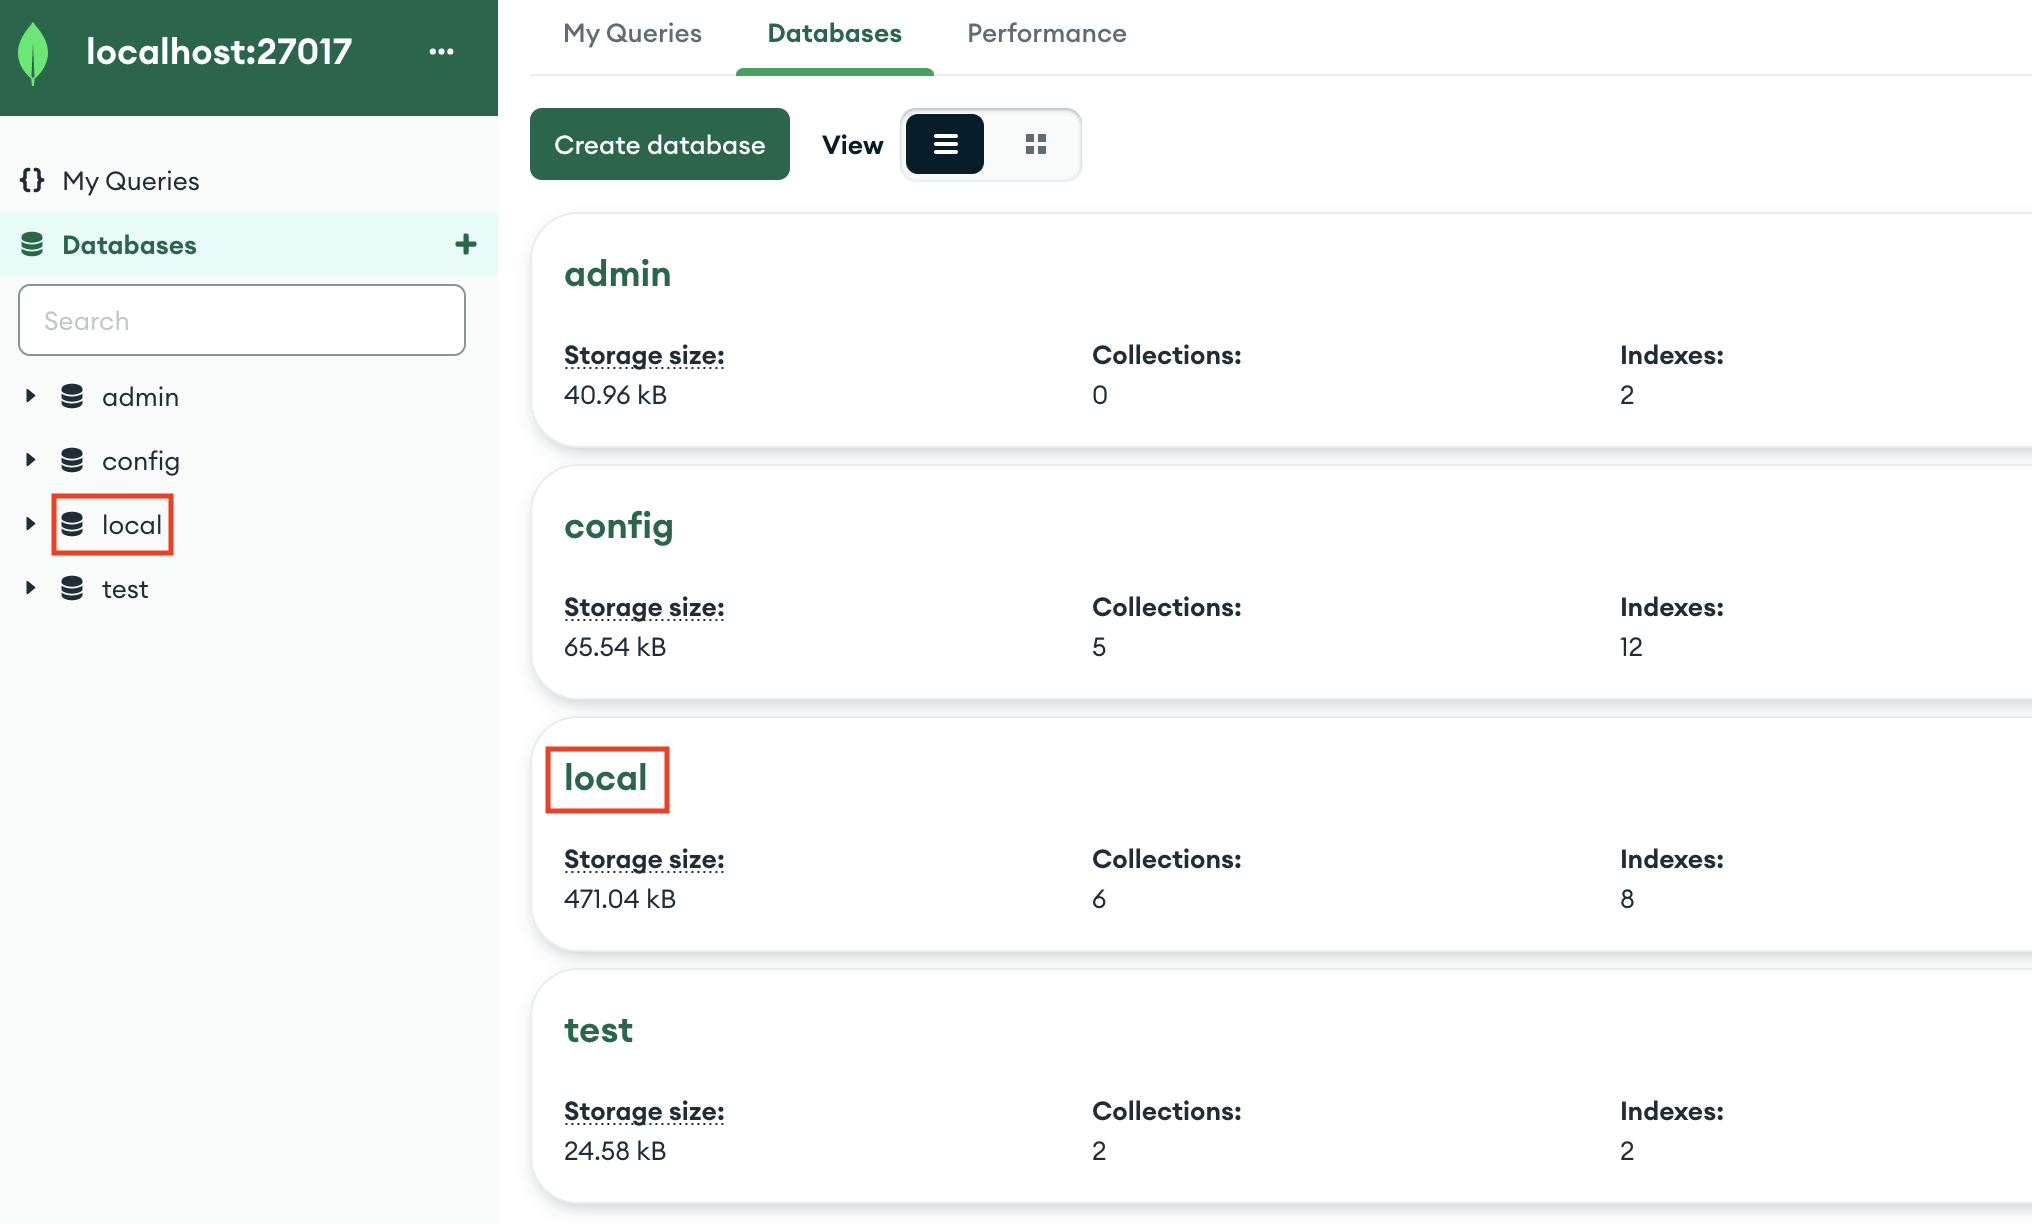
\includegraphics[width=1.0\textwidth]{database}
    \caption{Datenbank in MongoDB Compass}
    \label{img:database}
\end{figure}

Lorem ipsum dolor sit amet, consetetur sadipscing elitr, sed diam nonumy eirmod tempor invidunt ut labore et dolore magna aliquyam erat, sed diam voluptua. At vero eos et accusam et justo duo dolores et ea rebum. Stet clita kasd gubergren, no sea takimata sanctus est Lorem ipsum dolor sit amet. Lorem ipsum dolor sit amet, consetetur sadipscing elitr, sed diam nonumy eirmod tempor invidunt ut labore et dolore magna aliquyam erat, sed diam voluptua. At vero eos et accusam et justo duo dolores et ea rebum. Stet clita kasd gubergren, no sea takimata sanctus est Lorem ipsum dolor sit amet.

\subsection{Entwicklung Echtzeit-Kommunikationsservice}

Lorem ipsum dolor sit amet, consetetur sadipscing elitr, sed diam nonumy eirmod tempor invidunt ut labore et dolore magna aliquyam erat, sed diam voluptua. At vero eos et accusam et justo duo dolores et ea rebum. Stet clita kasd gubergren, no sea takimata sanctus est Lorem ipsum dolor sit amet. Lorem ipsum dolor sit amet, consetetur sadipscing elitr, sed diam nonumy eirmod tempor invidunt ut labore et dolore magna aliquyam erat, sed diam voluptua. At vero eos et accusam et justo duo dolores et ea rebum. Stet clita kasd gubergren, no sea takimata sanctus est Lorem ipsum dolor sit amet.

\begin{figure}[H]
    \centering
    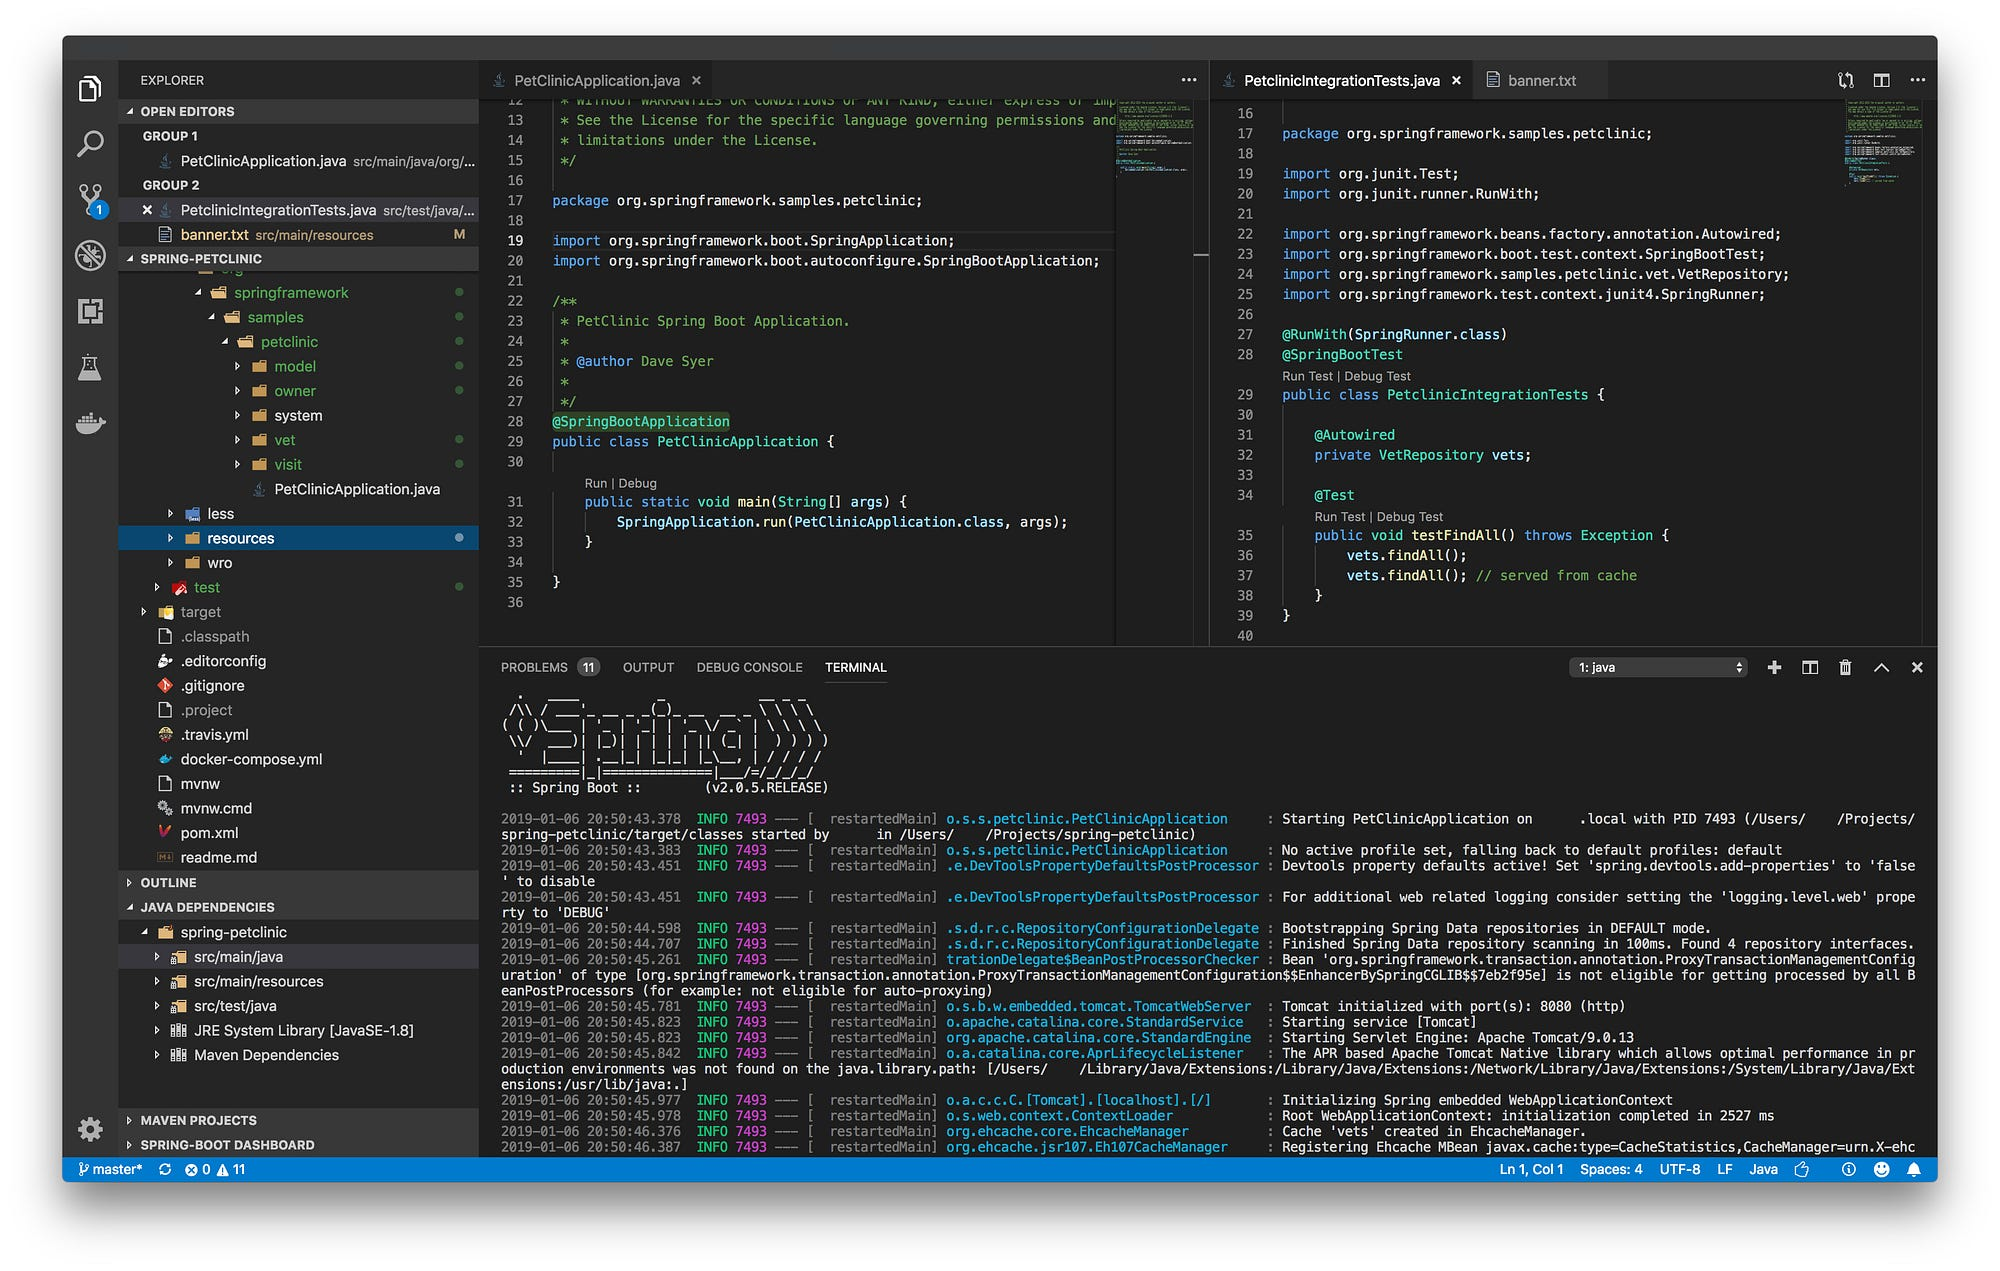
\includegraphics[width=1.0\textwidth]{spring}
    \caption{Codeauszug Backend-Service}
    \label{img:spring}
\end{figure}

Lorem ipsum dolor sit amet, consetetur sadipscing elitr, sed diam nonumy eirmod tempor invidunt ut labore et dolore magna aliquyam erat, sed diam voluptua. At vero eos et accusam et justo duo dolores et ea rebum. Stet clita kasd gubergren, no sea takimata sanctus est Lorem ipsum dolor sit amet. Lorem ipsum dolor sit amet, consetetur sadipscing elitr, sed diam nonumy eirmod tempor invidunt ut labore et dolore magna aliquyam erat, sed diam voluptua. At vero eos et accusam et justo duo dolores et ea rebum. Stet clita kasd gubergren, no sea takimata sanctus est Lorem ipsum dolor sit amet.


\section{Betrieb der Anwendung}

Die Anwendung wird in einem verwalteten Kubernetes-Cluster in AWS betrieben. Hierbei wurden verschiedene Services verwendet und wie folgt konfiguriert:
Lorem ipsum dolor sit amet, consetetur sadipscing elitr, sed diam nonumy eirmod tempor invidunt ut labore et dolore magna aliquyam erat, sed diam voluptua. At vero eos et accusam et justo duo dolores et ea rebum. Stet clita kasd gubergren, no sea takimata sanctus est Lorem ipsum dolor sit amet. Lorem ipsum dolor sit amet, consetetur sadipscing elitr, sed diam nonumy eirmod tempor invidunt ut labore et dolore magna aliquyam erat, sed diam voluptua. At vero eos et accusam et justo duo dolores et ea rebum. Stet clita kasd gubergren, no sea takimata sanctus est Lorem ipsum dolor sit amet.
\begin{figure}[H]
    \centering
    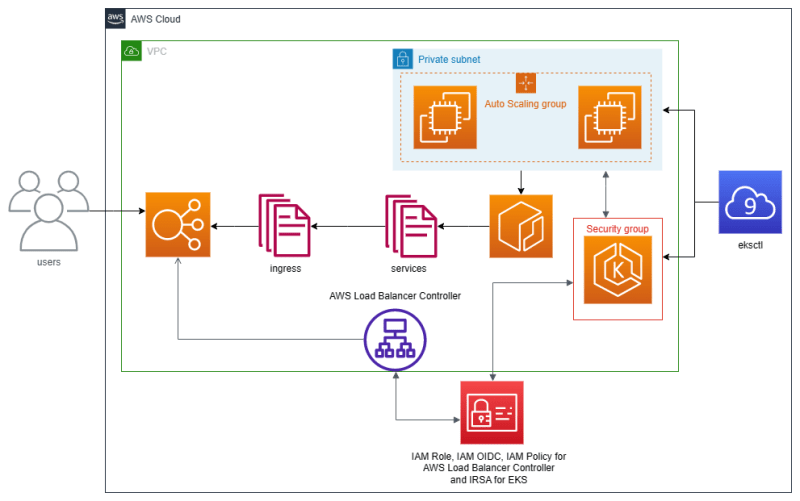
\includegraphics[width=1.0\textwidth]{EKS}
    \caption{Umsetzung manged Kubernetes}
    \label{img:EKS}
\end{figure}

Lorem ipsum dolor sit amet, consetetur sadipscing elitr, sed diam nonumy eirmod tempor invidunt ut labore et dolore magna aliquyam erat, sed diam voluptua. At vero eos et accusam et justo duo dolores et ea rebum. Stet clita kasd gubergren, no sea takimata sanctus est Lorem ipsum dolor sit amet. Lorem ipsum dolor sit amet, consetetur sadipscing elitr, sed diam nonumy eirmod tempor invidunt ut labore et dolore magna aliquyam erat, sed diam voluptua. At vero eos et accusam et justo duo dolores et ea rebum. Stet clita kasd gubergren, no sea takimata sanctus est Lorem ipsum dolor sit amet.









\newpage
\chapter{Evaluation} 
Lorem ipsum dolor sit amet, consetetur sadipscing
elitr, sed diam nonumy eirmod tempor invidunt ut labore
et dolore magna aliquyam erat, sed diam voluptua. At vero eos et
accusam et justo duo dolores et ea rebum. Stet clita kasd gubergren, 
no sea takimata sanctus est Lorem ipsum dolor sit amet. Lorem ipsum dolor 
sit amet, consetetur sadipscing elitr, sed diam nonumy eirmod tempor 
invidunt ut labore et dolore magna aliquyam erat, sed diam voluptua. 
At vero eos et accusam et justo duo dolores et ea rebum. Stet clita kasd 
gubergren, no sea takimata sanctus est Lorem ipsum dolor sit amet.

\section{Ergebnis der Anforderungsanalyse}


Nutzer können sich über die Anwendung anmelden und registrieren. Eine Registrierung ist ausschließlich möglich, wenn der Benutzer von einer Organisation eingeladen wurde. Der Authentifizierungsprozess verläuft in beiden Komponenten weitgehend identisch. Der Benutzer führt die Authentifizierung über einen zentralen OpenID-Provider im EKS-Cluster durch \textbf{(FA\#01)}.

Lorem ipsum dolor sit amet, consetetur sadipscing elitr, sed diam nonumy eirmod tempor invidunt ut labore et dolore magna aliquyam erat, sed diam voluptua. \textbf{(FA\#02)}.
At vero eos et accusam et justo duo dolores et ea rebum. Stet clita kasd gubergren, no sea takimata sanctus est Lorem ipsum dolor sit amet. \textbf{(FA\#03)}.
Lorem ipsum dolor sit amet, consetetur sadipscing elitr, sed diam nonumy eirmod tempor invidunt ut labore et dolore magna aliquyam erat, sed diam voluptua. \textbf{(FA\#04)}.
At vero eos et accusam et justo duo dolores et ea rebum. Stet clita kasd gubergren, no sea takimata sanctus est Lorem ipsum dolor sit amet. \textbf{(FA\#05)}.


Das System startet in der Pilotphase mit vergleichsweise wenigen Nutzern, erfordert jedoch dennoch eine stabile und zuverlässige Verbindung. Die Anzahl der Nutzer kann durch den Abschluss neuer Verträge schnell stark ansteigen, weshalb eine flexible Skalierung der Anwendung durch den Einsatz von EKS gewährleistet wird \textbf{(NFA\#01)}.

Lorem ipsum dolor sit amet, consetetur sadipscing elitr, sed diam nonumy eirmod tempor invidunt ut labore et dolore magna aliquyam erat, sed diam voluptua \textbf{(NFA\#02)}.
At vero eos et accusam et justo duo dolores et ea rebum. Stet clita kasd gubergren, no sea takimata sanctus est Lorem ipsum dolor sit amet \textbf{(NFA\#03)}.
Lorem ipsum dolor sit amet, consetetur sadipscing elitr, sed diam nonumy eirmod tempor invidunt ut labore et dolore magna aliquyam erat, sed diam voluptua \textbf{(NFA\#04)}.
At vero eos et accusam et justo duo dolores et ea rebum. Stet clita kasd gubergren, no sea takimata sanctus est Lorem ipsum dolor sit amet \textbf{(NFA\#05)}.


\section{Test Einsatz der Software}

Beim ersten Testlauf der Software wurde ein Rettungsdiensteinsatz in einer realen Umgebung simuliert. Dabei wurde ein Szenario gewählt, das einen häufig auftretenden Vorfall darstellen sollte. In diesem Szenario gab es einen 45-jährigen männlichen Patienten mit allergischem Schock und einen Sturz einer 85-jährigen Frau. Das Ziel des Testlaufs bestand darin, die Einsätze mit begrenzten Notarztressourcen möglichst schnell abzuarbeiten und dabei alle Standards im Rettungsdienst einzuhalten. Die Einsätze wurden zweimal simuliert: einmal unter Verwendung der TNA-Software und einmal auf dem herkömmlichen Versorgungsweg.
\\\\
\textbf{Ablauf des Einsatzverlaufs nach dem klassischen Modell:}
\\\\
\textbf{Alarmierung I:}
Um 8:00 Uhr ging in der örtlichen Leitstelle ein Alarm für einen männlichen Patienten mit allergischem Schock ein. Die Rettungsfahrzeuge RTW \& NEF rückten um 8:04 Uhr aus. Die Besatzung bestand aus 2 Notfallsanitätern, einem Rettungssanitäter (Fahrer) und einem Notarzt, die auf dem Weg zum Einsatzort waren.
\\\\
\textbf{Eintreffen am Einsatzort:}
Der RTW traf als Erstes um 8:10 Uhr am Einsatzort ein, das NEF befand sich weiterhin auf der Anfahrt. Die Notfallsanitäter diagnostizierten den Schock und bereiteten die Verabreichung eines Medikaments vor. Die Freigabe zur Verabreichung von Medikamenten darf nur durch einen Arzt erfolgen.
Der Notarzt traf um 08:15 Uhr am Einsatzort ein und bestätigte die Freigabe zur Medikamentenverabreichung.
\\\\
\textbf{Alarmierung II:}
Es ging eine Alarmierung für eine gestürzte 85-jährige Patientin ein. Ein RTW mit einer anderen Besatzung, bestehend aus 2 Notfallsanitätern, rückte zum Einsatzort aus.
\\\\
\textbf{Eintreffen am Einsatzort:}
Die Besatzung traf um 8:20 Uhr am Einsatzort ein und stellte eine schwerwiegende Verletzung fest. Sie benötigten dringend die fachliche Unterstützung eines Notarztes.
Der Notarzt war derzeit bei einem anderen Einsatz gebunden und beendete diesen so schnell wie möglich. Anschließend begab er sich zur nächsten Einsatzstelle und traf um 8:27 Uhr bei der Patientin ein. Der Arzt diagnostizierte die Verletzung, und die Patientin wurde in die nächstgelegene Klinik transportiert.
\\\\
Beide Einsätze konnten innerhalb von 30 Minuten abgeschlossen werden.
\\\\
\textbf{Ablauf des Einsatzverlaufs unter Verwendung der TNA-Software:}
\\\\
\textbf{Alarmierung I:}
Um 8:00 Uhr ging in der örtlichen Leitstelle ein Alarm für einen männlichen Patienten mit allergischem Schock ein. Die Rettungsfahrzeuge RTW \& NEF rückten um 8:04 Uhr aus. Die Besatzung bestand aus 2 Notfallsanitätern und einem Rettungssanitäter (Fahrer). Der Notarzt war nicht physisch im Fahrzeug anwesend, sondern wurde in den Einsatz über die TNA-Software aus der Ferne alarmiert.
\\\\
\textbf{Eintreffen am Einsatzort:}
Der RTW traf um 8:10 Uhr als Erstes am Einsatzort ein. Die Notfallsanitäter diagnostizierten den Schock und bereiteten die Verabreichung eines Medikaments vor. Die Freigabe zur Verabreichung von Medikamenten erfolgte sofort durch den Notarzt, der dies über die TNA-Software koordinierte, überwachte und rechtssicher dokumentierte.
\\\\
\textbf{Alarmierung II:}
Es ging eine Alarmierung für eine gestürzte 85-jährige Patientin ein. Ein RTW mit einer anderen Besatzung, bestehend aus 2 Notfallsanitätern, rückte zum Einsatzort aus.
\\\\
\textbf{Eintreffen am Einsatzort:}
Die Besatzung traf um 8:20 Uhr am Einsatzort ein und stellte eine schwerwiegende Verletzung fest. Sie benötigten dringend die fachliche Unterstützung eines Notarztes. Die Besatzung forderte ein Telekonsil über die TNA-Software an. Der Notarzt öffnete um 8:23 Uhr eine Videoverbindung, um die Patientin zu begutachten. Anschließend wurden Maßnahmen vor Ort durch das Team eingeleitet, die vom Notarzt delegiert wurden.
\\\\
Beide Einsätze wurden innerhalb von 30 Minuten abgeschlossen. Der Arbeitsaufwand für den Notarzt betrug dabei jedoch weniger als 5 Minuten.
\\\\
In Bezug auf die Behandlungsqualität konnten keine Unterschiede festgestellt werden. Die Freigabe des Medikaments konnte problemlos aus der Ferne erfolgen. Im zweiten Fall, bei der Diagnose der Verletzung über die Kamera, war der Video-Livestream ausreichend klar, um schnell eine Entscheidung zu treffen.

Das durchgespielte Szenario wurde anschließend mehrfach wiederholt, wobei der Standort des Arztes angepasst wurde. Der Arzt wurde sowohl in der Leitstelle als auch in der Klinik positioniert, um zu prüfen, ob er neben seiner Telenotarzttätigkeit zusätzlichen Aufgaben in der Klinik nachgehen kann. Es konnte jedoch keine signifikante Verbesserung festgestellt werden. Wenn der Notarzt in der Klinik an Patienten gebunden ist, leidet die Qualität der präklinischen Notfallversorgung.
\newpage
\chapter{Zusammenfassung und Ausblick}
Lorem ipsum dolor sit amet, consetetur sadipscing
elitr, sed diam nonumy eirmod tempor invidunt ut labore
et dolore magna aliquyam erat, sed diam voluptua. At vero eos et
accusam et justo duo dolores et ea rebum. Stet clita kasd gubergren, 
no sea takimata sanctus est Lorem ipsum dolor sit amet. Lorem ipsum dolor 
sit amet, consetetur sadipscing elitr, sed diam nonumy eirmod tempor 
invidunt ut labore et dolore magna aliquyam erat, sed diam voluptua. 
At vero eos et accusam et justo duo dolores et ea rebum. Stet clita kasd 
gubergren, no sea takimata sanctus est Lorem ipsum dolor sit amet.

\section{Zusammenfassung}

Das Ziel dieser Arbeit war die Verbesserung der präklinischen Notfallversorgung, insbesondere die Bewältigung der hohen Ressourcenknappheit und die Optimierung der Patientenversorgung. Darüber hinaus sollte die Arbeit auch die Behandlung in der Klinik verbessern, indem eine Software entwickelt wird, die es auch einem Arzt in der Klinik ermöglicht, Patienten präklinisch zu behandeln. Zur Bestätigung der Hypothesen wurde im Rahmen dieser Arbeit eine Telenotarzt-Software entwickelt.

Zunächst wurden alle funktionalen und nicht-funktionalen Anforderungen für den Entwurf der Software gesammelt. Hierbei wurden insbesondere Anforderungen an die Skalierbarkeit und eine intelligente Möglichkeit zur Benutzeranmeldung über verschiedene Systeme herausgestellt. Die Anforderungen wurden priorisiert und eingegrenzt.

In der Entwurfsphase wurden die Anforderungen zu einem detaillierten Softwareentwurf ausgearbeitet. Dabei wurden wichtige konzeptionelle Designentscheidungen im Detail untersucht und Einblicke in die gesamte Struktur der Software gewährt.

Anschließend erfolgte die Implementierung, bei der konkrete Verfahren zur Umsetzung der Software aufgezeigt wurden. Es wurden Code-Beispiele für bestimmte Stellen hervorgehoben und ein Verständnis für die Interoperabilität des Systems geschaffen.

In der Evaluationsphase wurde analysiert, ob die zuvor vereinbarten Anforderungen eingehalten werden konnten oder ob es Anforderungen gab, die nicht erfüllt werden konnten. Abschließend wurde die Software in einer Einsatzsimulation getestet und die Ergebnisse ausgewertet.

\section{Ausblick}

Die entwickelte Telenotarzt-Software hat bereits beeindruckende Fortschritte in der Verbesserung der präklinischen Notfallversorgung gezeigt. Diese Arbeit markiert jedoch erst den Beginn einer spannenden Entwicklung, die das Potenzial hat, die Art und Weise, wie medizinische Notfälle behandelt werden, grundlegend zu verändern. Im Weiteren werden vielversprechende Aspekte und zukünftige Entwicklungen in diesem Bereich skizziert.

Die Telenotarzt-Software kann in verschiedenen medizinischen Fachbereichen eingesetzt werden, um spezialisierte Notfallversorgung zu bieten. Dies könnte bedeuten, Experten aus Bereichen wie Neurologie, Kardiologie oder Kinderheilkunde einzubeziehen, um die präklinische Diagnose und Behandlung für spezifische Patientengruppen zu optimieren. Ebenso kann die Integration von Künstlicher Intelligenz zur Unterstützung von Telenotärzten die Effizienz und Genauigkeit der Diagnosen und Behandlungspläne weiter steigern. KI kann in Echtzeit Daten analysieren und medizinisches Fachwissen zur Verfügung stellen, um schnelle Entscheidungsfindungen zu unterstützen.

Die kontinuierliche Überwachung und Qualitätssicherung der Telenotarzt-Software sowie die Schulung der beteiligten Fachkräfte sind von entscheidender Bedeutung. Dies schließt auch die Einbeziehung von Datenschutz- und Sicherheitsprotokollen ein, um den Schutz sensibler Gesundheitsdaten zu gewährleisten. Die zukünftige Zusammenarbeit mit verschiedenen Gesundheitssystemen, Krankenhäusern und Notfalldiensten erfordert die Schaffung von branchenübergreifenden Standards und die Gewährleistung der nahtlosen Interoperabilität zwischen verschiedenen Systemen und Plattformen.

Schließlich müssen ethische und rechtliche Aspekte berücksichtigt werden. Die Nutzung von Telenotarzt-Software wirft ethische und rechtliche Fragen auf, die weiter erforscht und adressiert werden müssen. Dies beinhaltet Fragen der Haftung, des Datenschutzes und der Einwilligung der Patienten.

Die Telenotarzt-Software hat das Potenzial, die Notfallmedizin zu revolutionieren und die Versorgung von Patienten in kritischen Situationen zu verbessern. Diese Arbeit hat wichtige Grundlagen gelegt, aber es bleibt noch viel zu tun, um diese Technologie weiterzuentwickeln und sicherzustellen, dass sie effektiv und verantwortungsbewusst eingesetzt wird. Die Zukunft der Telenotarzt-Software verspricht aufregende Entwicklungen, die das Gesundheitswesen nachhaltig beeinflussen werden.





% =========== Literaturverzeichnis =================
\newpage
\pagenumbering{Roman}
% =========== Abbildungsverzeichnis =================
\newpage
\addcontentsline{toc}{chapter}{\listfigurename}
\listoffigures


\newpage
\bibliographystyle{alphadin}
\addcontentsline{toc}{chapter}{Literatur- und Quellenverzeichnis}
% \bibliographystyle{unsrt}
\bibliography{LiteraturTest}


\addchap{Anhang}
Lorem ipsum dolor sit amet, consetetur sadipscing
elitr, sed diam nonumy eirmod tempor invidunt ut labore
et dolore magna aliquyam erat, sed diam voluptua. At vero eos et
accusam et justo duo dolores et ea rebum. Stet clita kasd gubergren, 
no sea takimata sanctus est Lorem ipsum dolor sit amet. Lorem ipsum dolor 
sit amet, consetetur sadipscing elitr, sed diam nonumy eirmod tempor 
invidunt ut labore et dolore magna aliquyam erat, sed diam voluptua. 
At vero eos et accusam et justo duo dolores et ea rebum. Stet clita kasd 
gubergren, no sea takimata sanctus est Lorem ipsum dolor sit amet. 


\end{document}

